\chapter{The Relative Importance of Sire and Dam}
\label{cha:Lush_Chapter_29}
\index{Fertility|(}
\index{Sex linkage|(}
\index{Sire, importance compared with dam|(}

In general, sire and dam are equally important in inheritance.
There are three exceptions which are sometimes of practical importance.
The first is that a sire can have many more offspring in a single
season.\footnote{Monogamous species, such as pigeons, doves, and some
foxes, are exceptions to this. Among them the sire generally leaves about
the same number of offspring as the dam.} Therefore, the sire is much more
important than any one dam in determining the inheritance of the next
generation in the herd, although not more important in determining the
inheritance of any one animal. This is the basis for the common statement
that ``The sire is half the herd.''\footnote{This statement is an
exaggeration in the many cases where a sire is kept in service for less
than the average length of a generation. For example, in small dairy
herds, one sire is rarely used much more than two years; but the average
productive life of the cows is more nearly four years. Rarely are more
than half the cows in a herd daughters of one bull. Only half of their
genes come from him; hence one sire rarely furnishes more than a fourth
of the genes of the whole herd, although he does furnish half of the genes
of his own offspring.} The second exception is sex-linked inheritance. The
general rule in sex-linked inheritance is that sons are more like their
dams, and daughters are more like their sires than in ordinary inheritance.
The third exception is the one already discussed in
Chapter~\ref{cha:Lush_Chapter_14} that where the merits of the two parents
are not equally well known, less attention should be paid to the less well
known one in estimating the merits or breeding value of their offspring.

\section*{HIGHER FERTILITY OF THE SIRE}

When a breeder with a one-sire herd buys a sire, he is buying half
the inheritance of many offspring. When he buys a dam he is buying
half the inheritance of her sons and daughters only. Therefore, he can
afford to spend more money to procure a desirable sire than to procure
an equally desirable female.

Every individual has as many female as male ancestors. Becau se of
the larger number of offspring per male used for breeding than per
female, it is the usual rule that a breed is influenced more by some of
its males than by any equal number of females. However, about half of
what the male transmits came to him from his dam. It occasionally
happens that a female will exert more influence on a breed than any
contemporary male. A notable case is that of the Holstein-Friesian cow,
De Kol 2nd, whose relationship to the whole breed (about 10 per cent)
is more than that of any other cow or bull. She is almost a great
grandam of the whole breed today.\footnote{\textit{Jour. of Heredity},
27:61--72.} Naturally she could not exert this
much influence by having an enormous number of calves, although she
did live at least 16 years and produced 14 calves. She exerted her
remarkable influence on the breed through the fact that she had five
different sons which were quite prominent sires of the breed in their
time and saw extended service in leading herds. At least four other sons
and one daughter also left registered descendants. This is an exceptional
case, yet it illustrates how a female may exert a tremendous influence
on a breed if several of her sons are saved for extensive use. There is
some reason for thinking that more improvement in the dairy breeds
can be accomplished by the careful selection of cows which are to be the
dams of sires and therefore the grandams of the next generation than
can be done directly by selecting among the bulls. However, the exact
balance of the quantitative relations involved here is not yet clear.
\index{Fertility|)}

\section*{SEX-LINKED INHERITANCE}

In all farm animals except poultry, so far as is yet known, the male
has an \textit{X} and a \textit{Y} chromosome and the female has two
\textit{X} chromosomes. In poultry this situation is reversed. The
discussion which follows may be applied to poultry by substituting
the other sex.

Genes carried by the \textit{Y} chromosomes would, of course, be
transmitted from sire to son in unbroken lines if there were no
crossing over between \textit{X} and \textit{Y}. It would not be easy
to distinguish the effects of such genes from secondary sexual
characteristics. It is unlikely that the \textit{Y} chromosomes can
often, if ever, be entirely empty, or they would have been lost long
ago without harm to the species. Yet genetic research has found only
a few genes on \textit{Y} chromosomes.

In some species of fish, in man, and perhaps in most mammals, some
parts of the \textit{X} chromosomes are homologous with parts of the
\textit{Y} chromosomes and these can cross over. Genes carried in these
regions show ``partial sex-linkage.''\index{Partial sex-linkage} Their behavior is intermediate
between that of autosomal genes and that of the completely sex-linked
genes which are carried on the nonhomologous parts of the \textit{X}
chromosome. The latter are meant when sex-linkage is discussed in the
following pages. Examples of partially sex-linked genes in man are
those for retinitis pigmentosa and those for \textit{total} color
blindness. The genes for the ordinary red-green color blindness are
completely sex-linked.

The genes carried on the \textit{X} chromosomes are those responsible for
sex-linked traits. The male receives all of his sex-linked genes from his
dam; and, so far as those genes are concerned, he is no relative at all of
his sire. The female receives half of her sex-linked genes from her dam
and half from her sire just as with her other genes. But her sire can only
transmit one kind of \textit{X} chromosome to her, whereas the dam can transmit
either one of the pair she has. So far as daughters are concerned, this
amounts to the same thing as if the sires were completely homozygous
for their sex-linked genes, whereas the dams are as heterozygous for sexlinked
genes as they are for other genes. Consequently, paternal half
sisters will receive from their sire identical sex-linked genes; but
maternal half sisters need not be any more like each other in sex-linked
genes than they are in other genes. The following pedigree diagrams of
the \textit{X} and \textit{Y} chromosome situation for males and for females show what
happens when this is extended to the grandparental generation. The
notes show the part which each grandparent plays in the sex-linked
inheritance of the grandson or granddaughter.

\begin{figure}
	\centering
    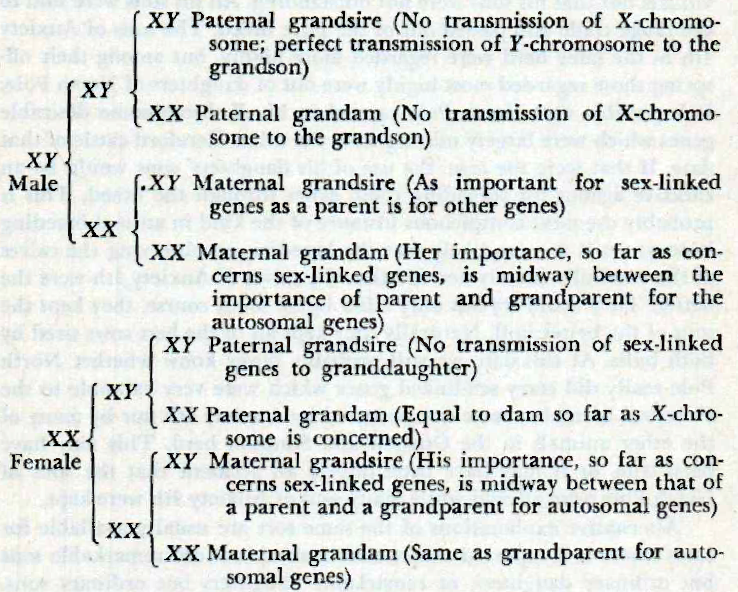
\includegraphics[width=\textwidth]{Page_353.png}
\end{figure}

If it is assumed, on the basis of chromosome number, that about 5
per cent of the genes are sex-linked, then the expected statistical
effects of sex-linkage are those shown in the last two columns of
Table~\ref{tbl:Lush_Table_20}. The existence of sex-linkage will have
so small an effect that for most characteristics it would be difficult
to prove that there is any sex-linkage. Differences in the correlations
observed between various kinds of relatives have sometimes been
interpreted as indicating sex-linkage, but it is rarely possible to be
sure that such differences were not caused by (1) sampling errors, (2)
greater similarity of environment for some kinds of relatives or (3)
differences in the selection which had been practiced for various kinds
of relatives. It is to be expected that there will be some sex-linkage
in the inheritance of most characteristics which are affected by many
genes but that only rarely will a large fraction of the genes be
sex-linked. In such rare cases the corrections will more nearly approach
those in columns 1 and 2 of Table~\ref{tbl:Lush_Table_20}. The main point
which Table~\ref{tbl:Lush_Table_20} demonstrates is that only rarely will
sex-linkage alter resemblances noticeably.

\begin{table}[htbp]
	\begin{center}
	\caption{\textsc{Expected Effects of Sex-Linkage on Correlations$^*$ Between Males or Females and Various of Their Relatives}}
	\label{tbl:Lush_Table_20}
	\begin{tabular}{L{5.24cm}|C{1.25cm}|C{1.25cm}|C{1.25cm}|C{1.25cm}|C{1.25cm}}
		\hline
		\hline
		~			& \multicolumn{2}{C{2.5cm}|}{All Genes}	 & No Sex- & \multicolumn{2}{C{2.5cm}}{5\% of Genes} \\
		~			& \multicolumn{2}{C{2.5cm}|}{Sex-linked} & linkage & \multicolumn{2}{C{2.5cm}}{Sex-linked}	  \\
		\cline{2-6}
		~						& ~		& ~			& Male or	& ~		& ~		    \\
		~						& Male	& Female	& Female	& Male	& Female	\\
		\hline
		\textit{Ancestors}				& ~		& ~		& ~		& ~		& ~		\\
		\hspace{1em}Sire 							& .00 	& .71 	& .50 	& .487	& .512	\\
		\hspace{1em}Dam 	 						& .71	& .50	& .50 	& .512	& .500	\\
		\hspace{1em}Paternal grandsire				& .00	& .00	& .25 	& .244	& .244	\\
		\hspace{1em}Paternal grandam				& .00	& .50	& .25	& .244	& .268	\\
		\hspace{1em}Maternal grandsire				& .50	& .35	& .25	& .268	& .256	\\
		\hspace{1em}Maternal grandam				& .35	& .25	& .25	& .256	& .250	\\
		\textit{Collateral relatives}	& ~		& ~		& ~		& ~		& ~		\\
		\hspace{1em}Full brother					& .50	& .35	& .50	& .500	& .494	\\
		\hspace{1em}Full sister						& .35	& .75	& .50	& .494	& .515	\\
		\hspace{1em}Paternal half brother			& .00	& .00	& .25	& .244	& .244	\\
		\hspace{1em}Paternal half sister			& .00	& .50	& .25	& .244	& .268	\\
		\hspace{1em}Maternal half brother			& .50	& .35	& .25	& .268	& .256	\\
		\hspace{1em}Maternal half sister			& .35	& .25	& .25	& .256	& .250	\\
		\textit{Half first cousin (female)}	& ~		& ~		& ~		& ~		& ~	\\
		\hspace{1em}Through paternal grandsire		& .00	& .00	& .062	& .061	& .061	\\
		\hspace{1em}Through paternal grandam		& .00	& .25	& .062	& .061	& .083	\\
		\hspace{1em}Through maternal grandsire		& .18	& .125	& .062	& .073	& .067	\\
		\hspace{1em}Through maternal grandam		& .09	& .062	& .062	& .064	& .062	\\
		\hline
	\end{tabular}
	\end{center}
	$^*$For traits entirely determined by heredity, without dominance or epistasis and in a population breeding at random.
\end{table}

In breed lore there are many cases where a sire was noted for his
daughters but not for his sons, or vice versa. In Hereford history it is
said that the daughters of North Pole were exceptionally good individuals
but that his sons were not outstanding. All his sons were sold to
the range trade and passed out of the pure breed. The sons of Anxiety
4th in the same herd were regarded more highly, but among their offspring
those regarded most highly were out of daughters of North Pole.
It is possible that North Pole carried in his \textit{X}-chromosome desirable
genes which were largely missing from the other Hereford cattle of that
date. If that were the case, the use of his daughters' sons would be an
effective agency for spreading those genes through the breed. This is
probably the most conspicuous instance of the kind in animal breeding
history; yet it is more likely that the breeders, on observing the calves
of the two bulls, merely decided that the calves of Anxiety 4th were the
better. They could try out only a few bulls; so, of course, they kept the
sons of the better bull. Naturally they kept all of the best cows sired by
both bulls. At this date we will probably never know whether North
Pole really did carry sex-linked genes which were very valuable to the
Hereford breed but were not possessed by Anxiety 4th nor by many of
the other animals in the Gudgell and Simpson herd. This may have
been true, or it may have been largely an accident that the sons of
North Pole were all sold while many sons of Anxiety 4th were kept.

Alternative explanations of the same sort are usually available for
cases where it is reported that a certain sire produced remarkable sons
but ordinary daughters, or remarkable daughters but ordinary sons.
Sex-linkage is a possible explanation in such cases, but it is probable
that the major factor has usually been the selection which the breeder
practiced and whether he was at that time selling many males to head
other herds or was selling only females.
\index{Sex linkage|)}

\section*{SUMMARY}

Because the sire can have so many more offspring per year than the
dam, he is a more important individual than any one female so far as
the whole herd is concerned, although not more important so far as
concerns any one offspring.

This makes it possible to cull prospective sires more closely than
prospective dams and profitable to pay more for an unusually good sire
than for an equally good dam.

Every individual has the same number of female and male ancestors.
A female who has more than two sons which are widely used may exert
more influence on a breed than any one of her sons. This has actually
happened at times, although most animals which have influenced a
breed much have been males.

Sex-linked inheritance has the effect of making daughters resemble
their sires, and sons resemble their dams, more closely than if there were
no sex-linkage. This is not often important.

Most cases reported from animal breeding history where a certain
sire produced good daughters but ordinary sons, or the reverse, are
probably to be explained as incidental results of the sales or culling
policy in that herd. Sex-linkage may have played a part in some of these
cases.

\nowidow
Sometimes one side of the pedigree will seem to be more important
than the other merely because more is known about it, and therefore
more use can be made of it for prediction.

\section*{REFERENCES}

\begin{hangparas}{0.5in}{1}%
Gowen, John W. 1924. Milk secretion. Baltimore: Williams and Wilkins. (This book
includes correlations between the performance of various female relatives in
the Holstein-Friesian Advanced Registry.)

Madsen, Karl. 1932. Inheritance of milking capacity. Nature, January 30.

Pearl, Raymond. 1922. The biology of death. Philadelphia: J. B. Lippincott Company.
(See pp. 174 and 175 for correlations between various kinds of relatives
in man. Six different characteristics are included.)

Smith, A. D. B., and Robison, 0. J. 1933. The genetics of cattle. Bibliographia
Genetica X. (See pp. 46--51 for a review of the evidence on sex-linkage in the
inheritance of milk and fat production.)

Snyder, Laurence H. 1942. The mutant gene in man. Amer. Nat. 76:131--33.

Winge, O. 1934. The experimental alteration of sex chromosomes into autosomes
and vice versa, as illustrated by Lebistes. Comp. Rend. Laboratoire Carlsberg,
21:1--49. (An account of the sex-chromosome situation in this genus of
fish with much about sex-linked genes and about crossing over between the
\textit{X} and \textit{Y} chromosomes.)
\end{hangparas}
\index{Sire, importance compared with dam|)}